\chapter{IMPLEMENTASI} \label{chap:implementasi}

\tab Pada bab ini dijelaskan mengenai implementasi dari perancangan struktur data dan algoritme untuk menyelesaikan permasalahan \problemDua{} sebagaimana yang telah dijelaskan pada Bab \ref{chap:analisis-perancangan-sistem}. Penjelasan implementasi terdiri dari penjelasan kelas dan fungsi yang dibuat, disertai dengan \textit{pseudocode} untuk masing-masing fungsi tersebut.

\section{Lingkungan Implementasi}
\tab Lingkungan implementasi dalam pembuatan Tugas Akhir ini meliputi perangkat keras dan perangkat lunak dengan spesifikasi sebagai berikut:

\begin{enumerate}
	\item Perangkat keras:
	\begin{itemize}
		\item Prosesor 2.6 GHz Intel Core i5 (I5-4278U)
		\item Memori 8 GB 1600 MHz DDR3
	\end{itemize}
	\item Perangkat lunak:
	\begin{itemize}
		\item Sistem operasi macOS Mojave Versi 10.14.5
		\item \textit{Text editor} Visual Studio Code Versi 1.33.1
		\item Bahasa Pemrograman Python 3.7.3
	\end{itemize}			
\end{enumerate}

\section{Implementasi \textit{Data Precomputing}}
\tab \textit{Data precomputing} merupakan pemrosesan tahap pertama dalam algoritme k-MPPTI yang bertujuan untuk mengolah \textit{dataset} produk $P$ dan preferensi pelanggan $C$ dengan jumlah data sebanyak $n$ dan ukuran dimensi sebesar $d$, menjadi sebuah $Pandora Box$ yang menyimpan skor kontribusi pasar semua produk pada setiap waktu. 

Algoritme ini diimplementasikan menggunakan paradigma pemrograman berorientasi objek, sehingga semua data dan fungsi dibungkus dalam kelas-kelas. Ada empat macam kelas yang diimplementasikan, yaitu kelas \textit{EventQueue}, \textit{PandoraBox}, \textit{ReverseSkyline}, dan \textit{DynamicSkyline}. 

\begin{figure}[H]
	\begin{algorithm}[H]
		\caption{Precomputing}
		\begin{algorithmic}[1]
			\Statex \textbf{Input \hskip1em :} product dataset $P$, customer dataset $C$ 
			\Statex \textbf{Output \hskip0.3em :} pandora box $PB$
			\State $EQ \leftarrow$ init event queue 
			\State $D \leftarrow$ data indexing $P, C$ 
			\ForAll {$d \in D$}
			\State $EQ \leftarrow$ enqueue $d$
			\EndFor
			\State sort $EQ$
			\State $PA \leftarrow \emptyset$ of active products
			\State $CA \leftarrow \emptyset$ of active customers
			\State $PB \leftarrow$ init pandora box
			\State $RSL \leftarrow$ init reverse skyline
			\State $DSL \leftarrow$ init dynamic skyline
			\algstore{main1}
		\end{algorithmic}
	\end{algorithm}
	\caption{Algoritme \textit{precomputing} (bagian 1) \label{algo:main-func-1}}
\end{figure}

Secara garis besar, langkah yang dilakukan selama \textit{precomputing} adalah (1) \textit{indexing} data dan pembentukan \textit{EventQueue} (\textit{psuedocode} baris 1-5 pada Algoritme \ref{algo:main-func-1}), (2) inisialisasi dan instansiasi objek (\textit{pseudocode} baris 6-10 pada Algoritme \ref{algo:main-func-1}), dan (3) pemrosesan \textit{event} (\textit{pseudocode} baris 11-36 pada Algoritme \ref{algo:main-func-2}).

\begin{figure}[H]
	\begin{algorithm}[H]
		\caption{Precomputing}
		\begin{algorithmic}[1]
			\algrestore{main1}
			\While {$EQ$ is not empty}
			\State $e \leftarrow$ dequeue $EQ$
			\If {$e$ role is product}
			\If {$e$ action is insertion}  
			\State $PA \leftarrow$ append $p \in e$
			\State $RSL(p) \leftarrow$ compute reverse skyline
			\ForAll {$c \in RSL(p)$}
			\State $DSL(c) \leftarrow$ compute dynamic skyline
			\EndFor
			\ForAll {$c \in CA$}
			\State $PB \leftarrow$ update pandora box $DSL(c)$
			\EndFor
			\ElsIf {$e$ act is deletion}
			\ForAll {$c \in CA$}
			\State $PB \leftarrow$ update pandora box $DSL(c)$
			\EndFor
			\State $RSL(p) \leftarrow$ compute reverse skyline
			\ForAll {$c \in RSL(p)$}
			\State $DSL(c) \leftarrow$ find active child and
			\Statex \hspace{3.1cm} compute new dynamic skyline
			\EndFor
			\State $PA \leftarrow$ remove $p \in e$
			\EndIf
			\ElsIf{$e$ role is customer}
			\If {$e$ act is insertion} 
			\State $CA \leftarrow$ append $c \in e$ 
			\State $DSL(c) \leftarrow$ compute initial dynamic skyline
			\State $PB \leftarrow$ update pandora box $DSL(c)$
			\ElsIf {$e$ act is deletion}
			\State $PB \leftarrow$ update pandora box $DSL(c)$
			\State $CA \leftarrow$ remove $c \in e$ 
			\EndIf
			\EndIf
			\EndWhile
			\State export $PB$
		\end{algorithmic}
	\end{algorithm}
	\caption{Algoritme \textit{precomputing} (bagian 2) \label{algo:main-func-2}}
\end{figure}

\subsection{Kelas \textit{EventQueue}}
\tab Kelas \textit{EventQueue} mendefinisikan bentuk dan perilaku dari objek \textit{EQ} yang berfungsi untuk menyimpan \textit{event-event} yang terjadi di dalam himpunan data. \textit{EventQueue} tidak dibuat menggunakan struktur data \textit{queue} asli karena data yang digunakan adalah \textit{historical} dan harus diurutkan terlebih dahulu berdasarkan \textit{timestamp} dari masing-masing data. Sehingga, \textit{EventQueue} diimplementasikan menggunakan \textit{array} yang bekerja seperti \textit{queue}, yakni FIFO (\textit{First In First Out}). 

\begin{figure}[H]
	\begin{algorithm}[H]
		\caption{EventQueue Class}
		\begin{algorithmic}[1]
			\Statex \textbf{Input \hskip1em :} timestamp $t$, role $o$ (product/customer), data ID $id$, action $a$ (insertion/deletion)
			\Statex \textbf{Output \hskip0.3em :} event queue $E$
			\State $E \leftarrow \emptyset$
			\Procedure{$enqueue$}{$t$, $o$, $oid$, $a$}
			\State $e \leftarrow$ [$t, o, oid, a$]
			\State $E \leftarrow$ append $e$ 
			\EndProcedure
			\Procedure{$dequeue$}{}
			\State $e \leftarrow$ pop an element from $E$
			\State \Return $e$
			\EndProcedure
			\Procedure{$sortQueue$}{}
			\State $E \leftarrow$ sort elements in descending order based on sorting priority (timestamp, insertion act, deletion act, product, customer, data ID))
			\EndProcedure
		\end{algorithmic}
	\end{algorithm}
	\caption{Kelas \textit{EventQueue} \label{algo:event-queue-class}}
\end{figure}

\pagebreak
Ada tiga fungsi utama yang diimplementasikan, yaitu $enqueue$ untuk memasukkan data ke dalam \textit{array} pada indeks pertama, $dequeue$ untuk mengeluarkan data dari \textit{array} pada indeks terakhir; dan $sortQueue$ untuk mengurutkan data di dalam array.

\subsection{Kelas \textit{PandoraBox}}
\tab Kelas \textit{PandoraBox} mendefinisikan bentuk dan perilaku dari objek \textit{PB} yang berfungsi untuk menyimpan skor kontribusi pasar masing-masing produk $p \in P$ pada setiap waktu dalam interval hidupnya $t \in [t_i:t_e]$. \textit{PandoraBox} diimplementasikan menggunakan struktur data \textit{array} dua dimensi, yaitu ID produk dan \textit{timestamp}.

\begin{figure}[H]
	\begin{algorithm}[H]
		\caption{PandoraBox Class}
		\begin{algorithmic}[1]
			\Statex \textbf{Input \hskip1em :} $DSL(c)$, timestamp $ts$, probability score $pr$, last updated timestamp $lastts$, last probability score $lastpr$ 
			\Statex \textbf{Output \hskip0.3em :} filled pandora box $PB$
			\State $PB \leftarrow \emptyset$
			\Procedure{$updatePB$}{$DSL(c)$}
			\ForAll {$p \in DSL(c)$}
			\If{$ts > lastts$}
			\State $UpdateScore(p, ts, pr, lastts, lastpr)$
			\EndIf
			\State $PB(p, ts) \leftarrow PB(p, ts) + pr$  
			\EndFor
			\EndProcedure
			\Procedure{$updateScore$}{$p$, $ts$, $pr$, $lastts$, $lastpr$}
			\For {$i \leftarrow lastts+1$ to $ts$}
			\State $PB(p, i) \leftarrow PB(p, i) + lastpr$  
			\EndFor
			\EndProcedure
			\algstore{pbox}
		\end{algorithmic}
	\end{algorithm}
	\caption{Kelas \textit{PandoraBox} (bagian 1) \label{algo:pbox-class}}
\end{figure}

\pagebreak
Ada dua fungsi utama yang digunakan dalam proses \textit{data precomputing}, yaitu $updatePB$ untuk memperbarui skor kontribusi pasar pelanggan $c$ dan $updateScore$ untuk memperbarui indeks sebelumnya, jika ada yang kosong, menggunakan nilai probabilitas terakhir. Kelas \textit{PandoraBox} ditunjukkan oleh Algoritme \ref{algo:pbox-class}.

\begin{figure}[H]
	\begin{algorithm}[H]
		\caption{DynamicSkyline Class}
		\begin{algorithmic}[1]
			\Statex \textbf{Input \hskip1em :} customer $c$, active products $PA$, product in/out $p$
			\Statex \textbf{Output \hskip0.3em :} $DSL(p)$
			\Procedure{$computeDSL$}{$c$, $ts$, $act$, $p$}
			\If{$act$ is customer insertion} call $initDSL(c)$
			\ElsIf{$act$ is product insertion} call $productIn(c, p)$
			\ElsIf{$act$ is product deletion} call $productOut(c, p)$
			\EndIf
			\EndProcedure
			\Procedure{$productOut$}{$c$, $p$}
			\State $ac \leftarrow$ find active childs of $p$
			\State $DSL(c) \leftarrow$ call $productIn(c, ac)$  
			\State \Return $DSL(c)$
			\EndProcedure
			\algstore{dsl}
		\end{algorithmic}
	\end{algorithm}
	\caption{Kelas \textit{DynamicSkyline} (bagian 1) \label{algo:dsl1}}
\end{figure}

\subsection{Kelas \textit{Dynamic Skyline}}
\tab Kelas \textit{DynamicSkyline} mendefinisikan bentuk dan perilaku dari objek \textit{DSL} yang berfungsi untuk menangani komputasi \textit{dynamic skyline}, memiliki 3 jenis pemrosesan \textit{event}, yaitu (1) $initDSL$ yang dijalankan ketika ada data pelanggan yang masuk, ditunjukkan oleh \textit{pseudocode} baris 8-20 pada Algoritme \ref{algo:dsl2}; (2) $DSL-PI$ yang dijalankan ketika ada data produk yang masuk, ditunjukkan oleh \textit{pseudocode} baris 21-35 pada Algoritme \ref{algo:dsl2}; (3) $DSL-PD$ yang dijalankan ketika ada data produk yang keluar, ditunjukkan oleh \textit{pseudocode} baris 36-39 pada Algoritme \ref{algo:dsl2}.

\begin{figure}[H]
	\begin{algorithm}[H]
		\caption{DynamicSkyline Class}
		\begin{algorithmic}[1]
			\algrestore{dsl}
			\Procedure{$initDSl$}{$c$, $PA$}
			\State $CAND \leftarrow PA$
			\State sort $CAND$
			\For {$i \leftarrow$ 0 to length of $CAND$}
			\For {$j \leftarrow i + 1$ to length of $CAND$}
			\If {$p_i \prec_c p_j$} 
			\State add $p_j$ to the child list of $p_i$
			\State $CAND \leftarrow$ remove $p_j$
			\ElsIf {$p_j \prec_c p_i$} 
			\State add $p_i$ to the child list of $p_j$
			\State $CAND \leftarrow$ remove $p_i$
			\State \textbf{break} 
			\EndIf
			\EndFor
			\State \Return $CAND$ as $DSL(c)$
			\EndFor
			\EndProcedure
			\Procedure{$productIn$}{$c$, $p$}
			\State $CAND \leftarrow p$, current $DSL(c)$
			\State sort $CAND$
			\State $x \leftarrow$ get index of p in $CAND$
			\For {$i \leftarrow$ 0 to length of $CAND$}
			\If{$i < x$}
			\If {$p_i \prec_c p_{x}$} 
			\State add $p_x$ to the child list of $p_i$
			\State $CAND \leftarrow$ remove $p_x$
			\State \textbf{break}
			\EndIf
			\ElsIf{$i > x$}
			\If {$p_x \prec_c p_i$} 
			\State add $p_i$ to the child list of $p_x$
			\State $CAND \leftarrow$ remove $p_i$
			\EndIf
			\EndIf
			\EndFor
			\State \Return $CAND$ as $DSL(c)$
			\EndProcedure
		\end{algorithmic}
	\end{algorithm}
	\caption{Kelas \textit{DynamicSkyline} (bagian 2) \label{algo:dsl2}}
\end{figure}

\subsection{Kelas \textit{ReverseSkyline}}
\tab Kelas \textit{ReverseSkyline} mendefinisikan bentuk dan perilaku dari objek \textit{RSL} yang berfungsi untuk menangani komputasi \textit{reverse skyline}, meliputi (1) pembentukan \textit{orthant} pada fungsi $defineOrthant$ dan $getOrthantId$ yang ditunjukkan oleh \textit{pseudocode} baris 5-13 pada Algoritme \ref{algo:rsl2}, (2) menghitung semua \textit{midpoint} antara produk kueri dan setiap produk $p \in P$ pada fungsi $calcMidpoint$ yang ditunjukkan pada \textit{pseudocode} baris 14-16 pada Algoritme \ref{algo:rsl2}, (3) menentukan \textit{midpoint skyline} masing-masing \textit{orthant} pada fungsi $findMidSkyline$ yang ditunjukkan oleh \textit{pseudocode} baris 17-30 pada Algoritme \ref{algo:rsl2}, dan (4) menentukan \textit{reverse skyline} pada fungsi $findReverseSkyline$ yang ditunjukkan oleh \textit{pseudocode} baris 31-38 pada Algoritme \ref{algo:rsl3}.

\begin{figure}[H]
	\begin{algorithm}[H]
		\caption{ReverseSkyline Class}
		\begin{algorithmic}[1]
			\Statex \textbf{Input \hskip1em :} product as query point $p_q$, active products $PA$, active customers $CA$, dimension of data $d$
			\Statex \textbf{Output \hskip0.3em :} $RSL(p)$
			\Procedure{$computeRSL$}{$p_q$}
			\State call $defineOrthant(d)$
			\State call $findMidSkyline(p_q, PA)$
			\State \Return $findReverseSkyline(CA)$
			\EndProcedure
			\Procedure{$defineOrthant$}{$d$}
			\For{$i \leftarrow 0$ to $2^d$}
			\State $id \leftarrow$ binary of $i$ 
			\State $o_{id} \leftarrow \emptyset$ 
			\EndFor
			\EndProcedure
			\algstore{rsl}
		\end{algorithmic}
	\end{algorithm}
	\caption{Kelas \textit{ReverseSkyline} (bagian 1) \label{algo:rsl1}}
\end{figure}

\begin{figure}[H]
	\begin{algorithm}[H]
		\caption{ReverseSkyline Class}
		\begin{algorithmic}[1]
			\algrestore{rsl}
			\Procedure{$getOrthantId$}{$D$}
			\For {\textbf{each} $i \in d$}
			\If {$D^i \leq p_q^i$} $id \leftarrow$ append $0$
			\Else {} $id \leftarrow$ append $1$
			\EndIf
			\EndFor
			\State \Return $id$
			\EndProcedure
			\Procedure{$calcMidpoint$}{$p_q$, $p$} 
			\For {\textbf{each} $i \in d$} $m \leftarrow$ $\frac{(p_q^i + p^i)}{2}$
			\EndFor
			\State \Return $m$
			\EndProcedure
			\Procedure{$findMidSkyline$}{$p_q, PA$}
			\ForAll {$p \in PA$}
			\If {$p \not= p_q$}
			\State $m \leftarrow CalcMidpoint(p_q, p)$ 
			\State $id \leftarrow GetOrthantId(p)$
			\If {$o_{id}$ is empty} $o_{id} \leftarrow m$
			\Else{} 
			\For {\textbf{each} $mc \in MSL(o_{id})$}
			\If{$m \prec_{p_q} mc$} 
			\State $MSL(o_{id}) \leftarrow$ delete $mc$
			\ElsIf{$mc \prec_{p_q} m$}
			\State \textbf{break} 
			\EndIf
			\EndFor
			\If{$\forall mc \in MSL(o_{id}) \nprec_{p_q} m$}
			\State $MSL(o) \leftarrow$ insert $m$
			\EndIf
			\EndIf
			\EndIf
			\EndFor
			\EndProcedure
			\Procedure{$findReverseSkyline$}{$p_q, CA$} 
			\For {$c \in CA$}
			\State $id \leftarrow$ $GetOrthantId(c)$
			\If {$o_{id}$ is empty} $RSL(p) \leftarrow$ insert $c$
			\Else{}  
			\If {$\forall m \in MSL(o_{id}) \nprec_{p_q} c$}
			\State $RSL(p) \leftarrow$ insert $c$
			\EndIf
			\EndIf
			\EndFor
			\State \Return $RSL(p)$
			\EndProcedure
		\end{algorithmic}
	\end{algorithm}
	\caption{Kelas \textit{ReverseSkyline} (bagian 2) \label{algo:rsl2}}
\end{figure}

\subsection{Metode Pengecekan Dominasi}

\tab Metode yang untuk pengecekan dominasi adalah dengan membandingkan selisih absolut data dengan titik kueri secara iteratif sejumlah dimensi data. Sehingga, semakin banyak dimensi data maka proses pengecekan dominasi semakin lama. Metode pengecekan dominasi ini digunakan dalam setiap komputasi \textit{dynamic skyline} dan \textit{reverse skyline}.

\begin{figure}[H]
	\begin{algorithm}[H]
		\caption{Check Domination}
		\begin{algorithmic}[1]
			\Statex \textbf{Input \hskip1em :} value of subject ($ob_1$), value of target ($ob_2$), value of query point ($ob_3$), dimension of data ($d$)
			\Statex \textbf{Output \hskip0.3em :} $ob_1 \prec_{ob_3} ob_2$ is true/false
			\Procedure{$isDominating$}{$ob_1, ob_2, ob_3$} 
			\State $dominating \leftarrow 0$ 
			\State $dominated \leftarrow 0$
			\For {\textbf{each} $i \in d$}
			\State $diff_1^i \leftarrow |ob_1^i - ob_3^i|$
			\State $diff_2^i \leftarrow |ob_2^i - ob_3^i|$
			\If {$diff_1^i = diff_2^i$}
			\State \textbf{continue}
			\ElsIf{$diff_1^i < diff_2^i$}
			\State $domininating \leftarrow dominating + 1$
			\ElsIf{$diff_1^i > diff_2^i$}
			\State $dominated \leftarrow dominated + 1$
			\EndIf
			\EndFor
			\If{$dominated = 0$ and $dominating \geq 1$} 
			\State \Return True
			\Else{} 
			\State \Return False
			\EndIf
			\EndProcedure
		\end{algorithmic}
	\end{algorithm}
	\caption{Fungsi cek dominasi \label{algo:check-dom}}
\end{figure}

\begin{figure}[H]
	\begin{algorithm}[H]
		\caption{Query Processing}
		\begin{algorithmic}[1]
			\Statex \textbf{Input \hskip1em :} Pandora Box $PB$, number of products $k$, time interval (time init $t_i$, time end $t_e$)
			\Statex \textbf{Output \hskip0.3em :} $k$ products
			\State $Q \leftarrow \emptyset$
			\ForAll {$p \in P$}
			\State $MC_p \leftarrow$ call $getScore(p, t_i, t_e)$
			\EndFor
			\State sort $MC$ in ascending order based on market contribution score
			\State $Q \leftarrow$ get top-k $MC$
		\end{algorithmic}
	\end{algorithm}
	\caption{Algoritme \textit{query processing} \label{algo:solution}}
\end{figure}

\begin{figure}[H]
	\begin{algorithm}[H]
		\caption{PandoraBox Class}
		\begin{algorithmic}[1]
			\algrestore{pbox}
			\Statex \textbf{Input \hskip1em :} product $p$, time interval (time init $t_i$, time end $t_e$)
			\Statex \textbf{Output \hskip0.3em :} total market contribution score $MC$
			\Procedure{$getScore$}{$p[id]$, $t_i$, $t_e$}
			\State $MC \leftarrow 0$ 
			\For {$i \leftarrow t_i$ to $t_e + 1$}
			\State $MC \leftarrow MC + PB(p, i)$
			\EndFor
			\Return $MC$
			\EndProcedure
		\end{algorithmic}
	\end{algorithm}
	\caption{Kelas \textit{PandoraBox} (bagian 2) \label{algo:pbox-class-2}}
\end{figure}

\section{Implementasi Algoritme \textit{Query Processing}}
\tab \textit{Query processing} merupakan pemrosesan tahap kedua dalam algoritme k-MPPTI yang bertujuan untuk memproses kueri yang dimasukkan oleh pengguna dengan memanfaatkan \textit{Pandora Box} dari hasil \textit{precomputing}. Proses diawali dengan mengakumulasi skor kontribusi pasar semua produk dalam interval waktu kueri, kemudian hasil akumulasi diurutkan dari yang terbesar. Langkah terakhir adalah mengembalikan hasil kueri berupa produk sejumlah $k$ beserta skor kontribusi pasarnya.

\section{Implementasi Antarmuka Pengguna}
\tab Antarmuka pengguna diimplementasikan menggunakan bahasa pemrograman Python, HTML, CSS, dan JavaScript, serta Flask sebagai kerangka kerja \textit{back-end}, Bootstrap sebagai kerangka kerja \textit{front-end}, dan pustaka Vis.js untuk menampilkan visualisasi data. 

Antarmuka pengguna memiliki empat menu utama yaitu, \textit{"Home"} sebagai halaman utama yang berisi pengenalan algoritme k-MPPTI, \textit{"Precompute"} untuk melakukan \textit{data precomputing}, \textit{"Search"} untuk melakukan pencarian $k$-produk yang paling diminati pelanggan dalam interval waktu tertentu, dan \textit{"Visualization"} untuk melihat visualisasi data.

Pada menu \textit{"Precompute"} (Gambar \ref{fig:precompute}), pengguna diberikan opsi untuk memasukkan data baru atau menggunakan \textit{session} yang sudah ada. Jika pengguna memasukkan data baru, artinya pengguna membuat \textit{session} baru dan data akan di-\textit{precompute} terlebih dahulu. Jika pengguna memilih session yang sudah ada, data tidak perlu di-\textit{precompute} ulang.

Setelah melalui proses \textit{precomputing}, pengguna dapat memasukkan kueri pencarian $k$-produk yang paling menjanjikan dalam interval waktu tertentu. Halaman web akan mengembalikan data berupa hasil kueri pencarian, yakni berupa ID produk dan skor kontribusi pasarnya sebagaimana yang ditunjukkan pada Gambar \ref{fig:search}.

\begin{figure}[H]
	\centering
	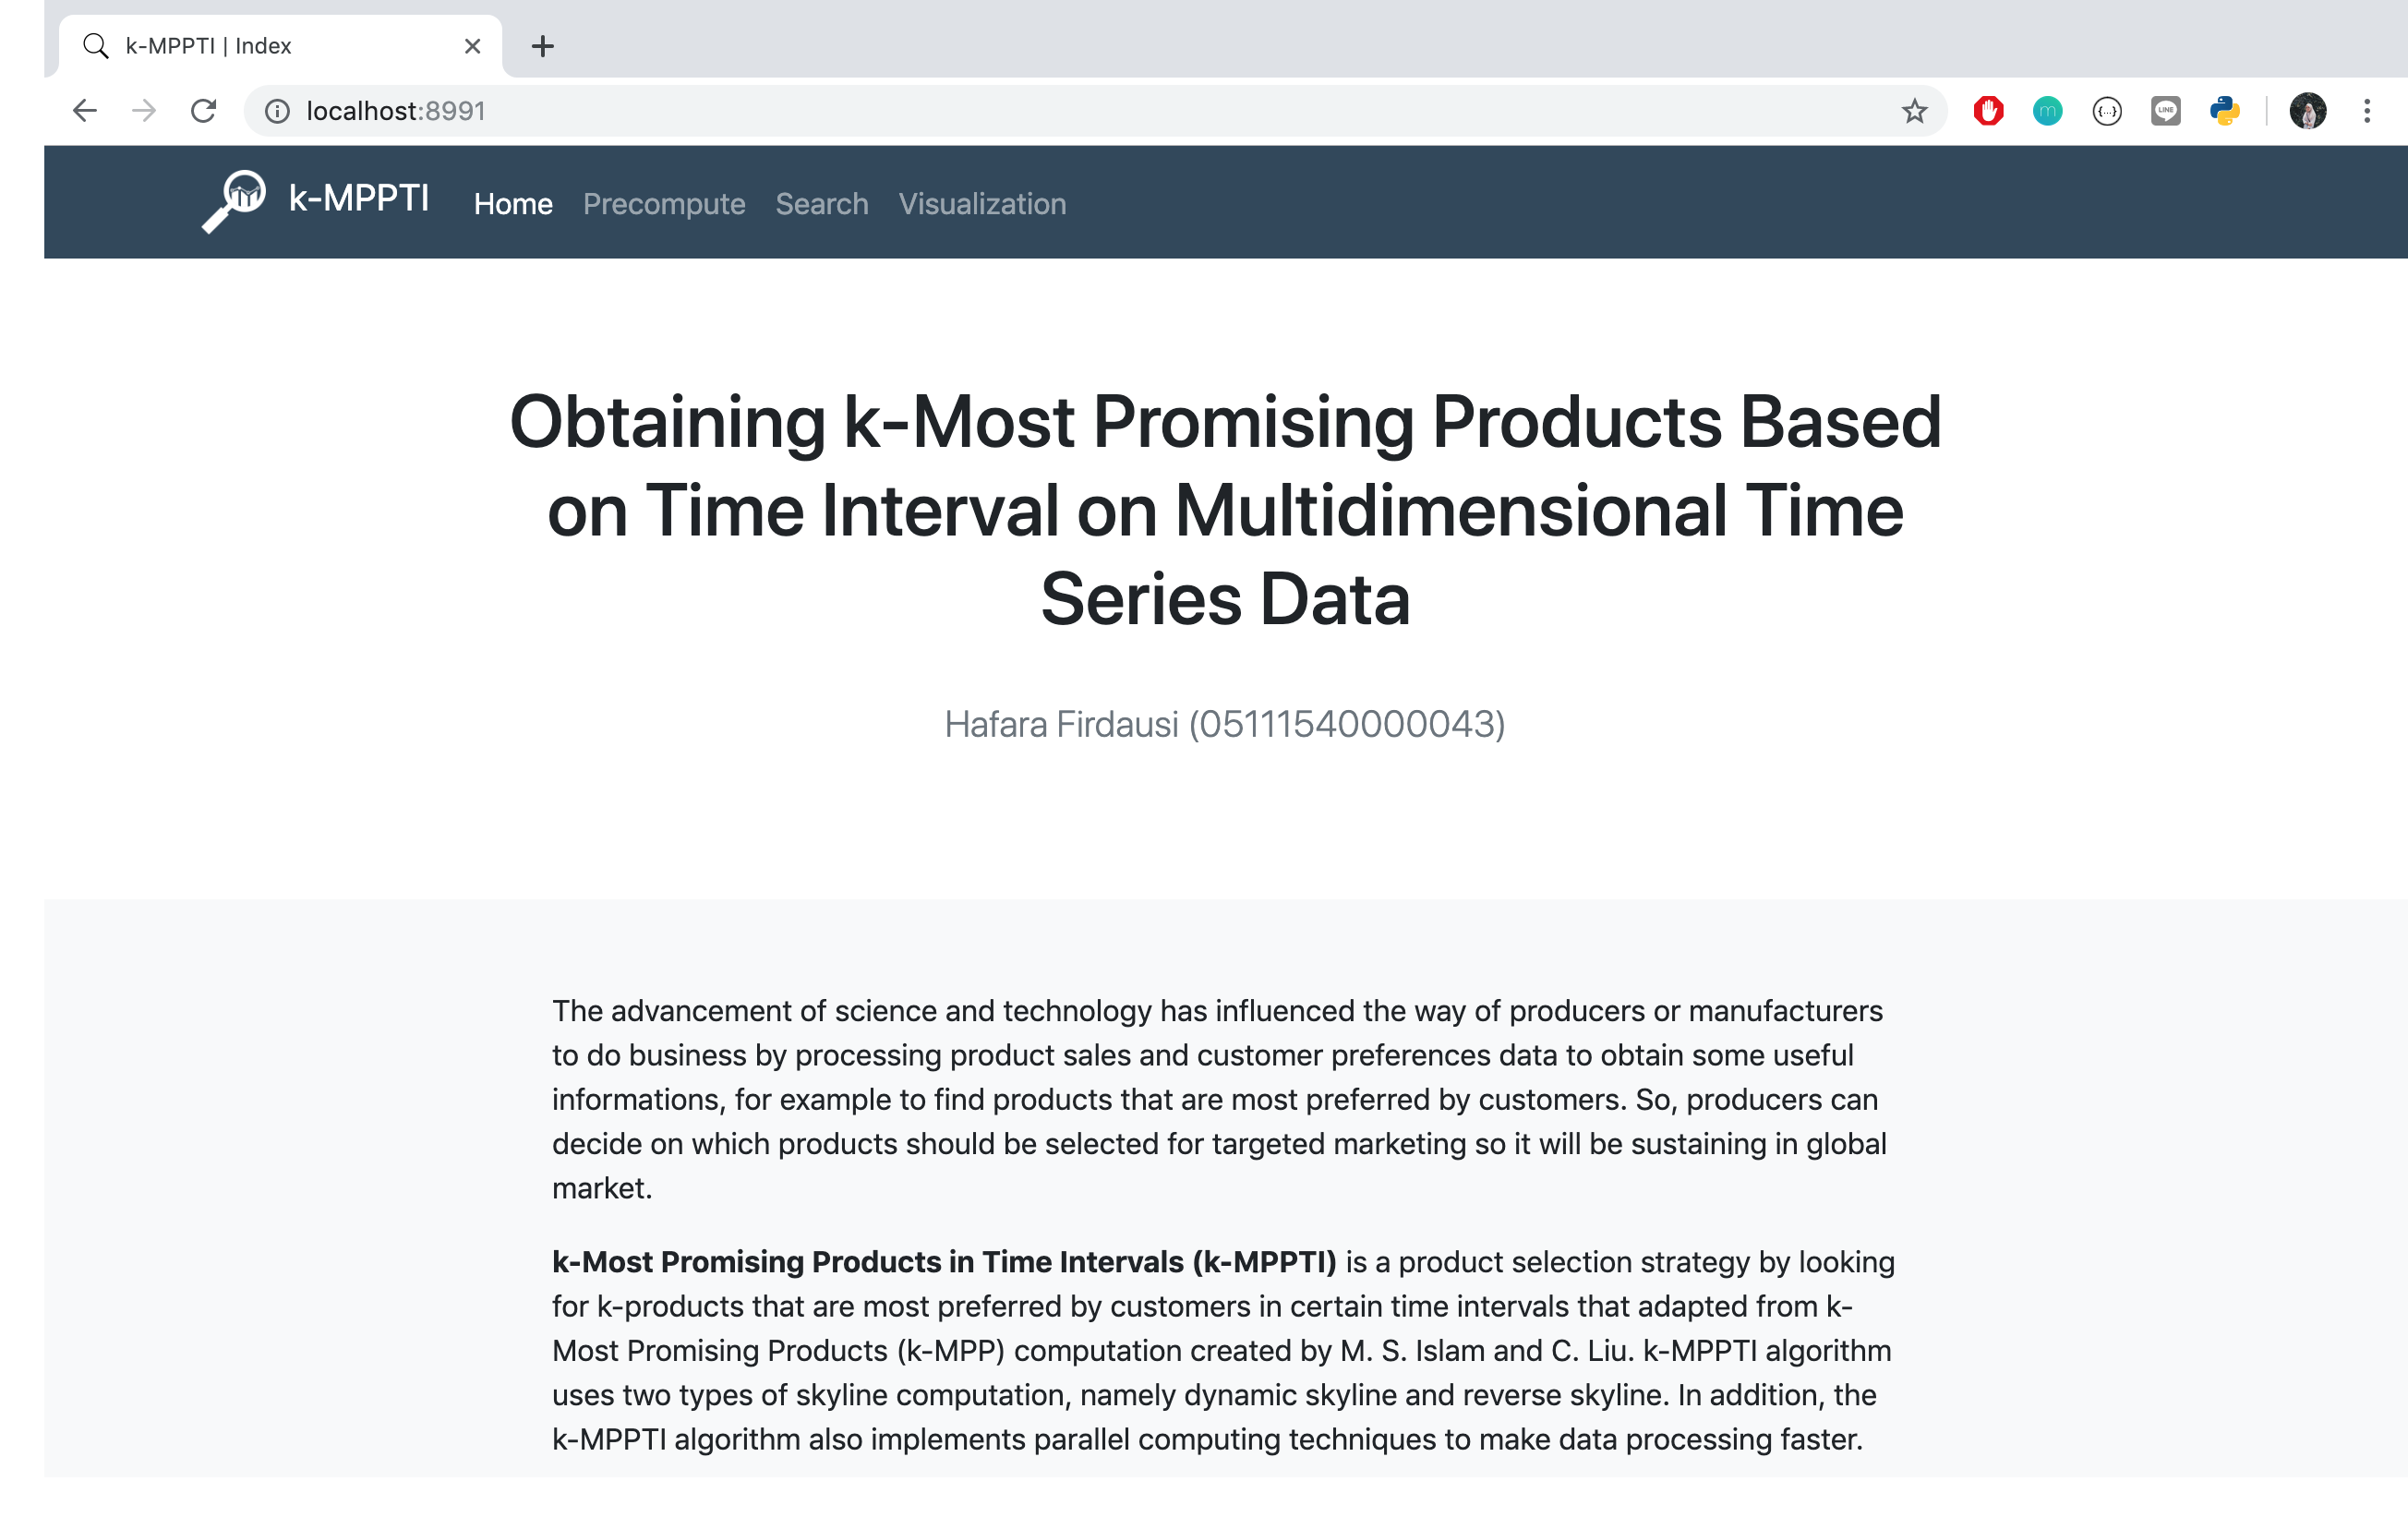
\includegraphics[width=10.5cm]{assets/img/bab4/home.png}
	\caption{Implementasi halaman \textit{Home}}
	\label{fig:home}
\end{figure}

\begin{figure}[H]
	\centering
	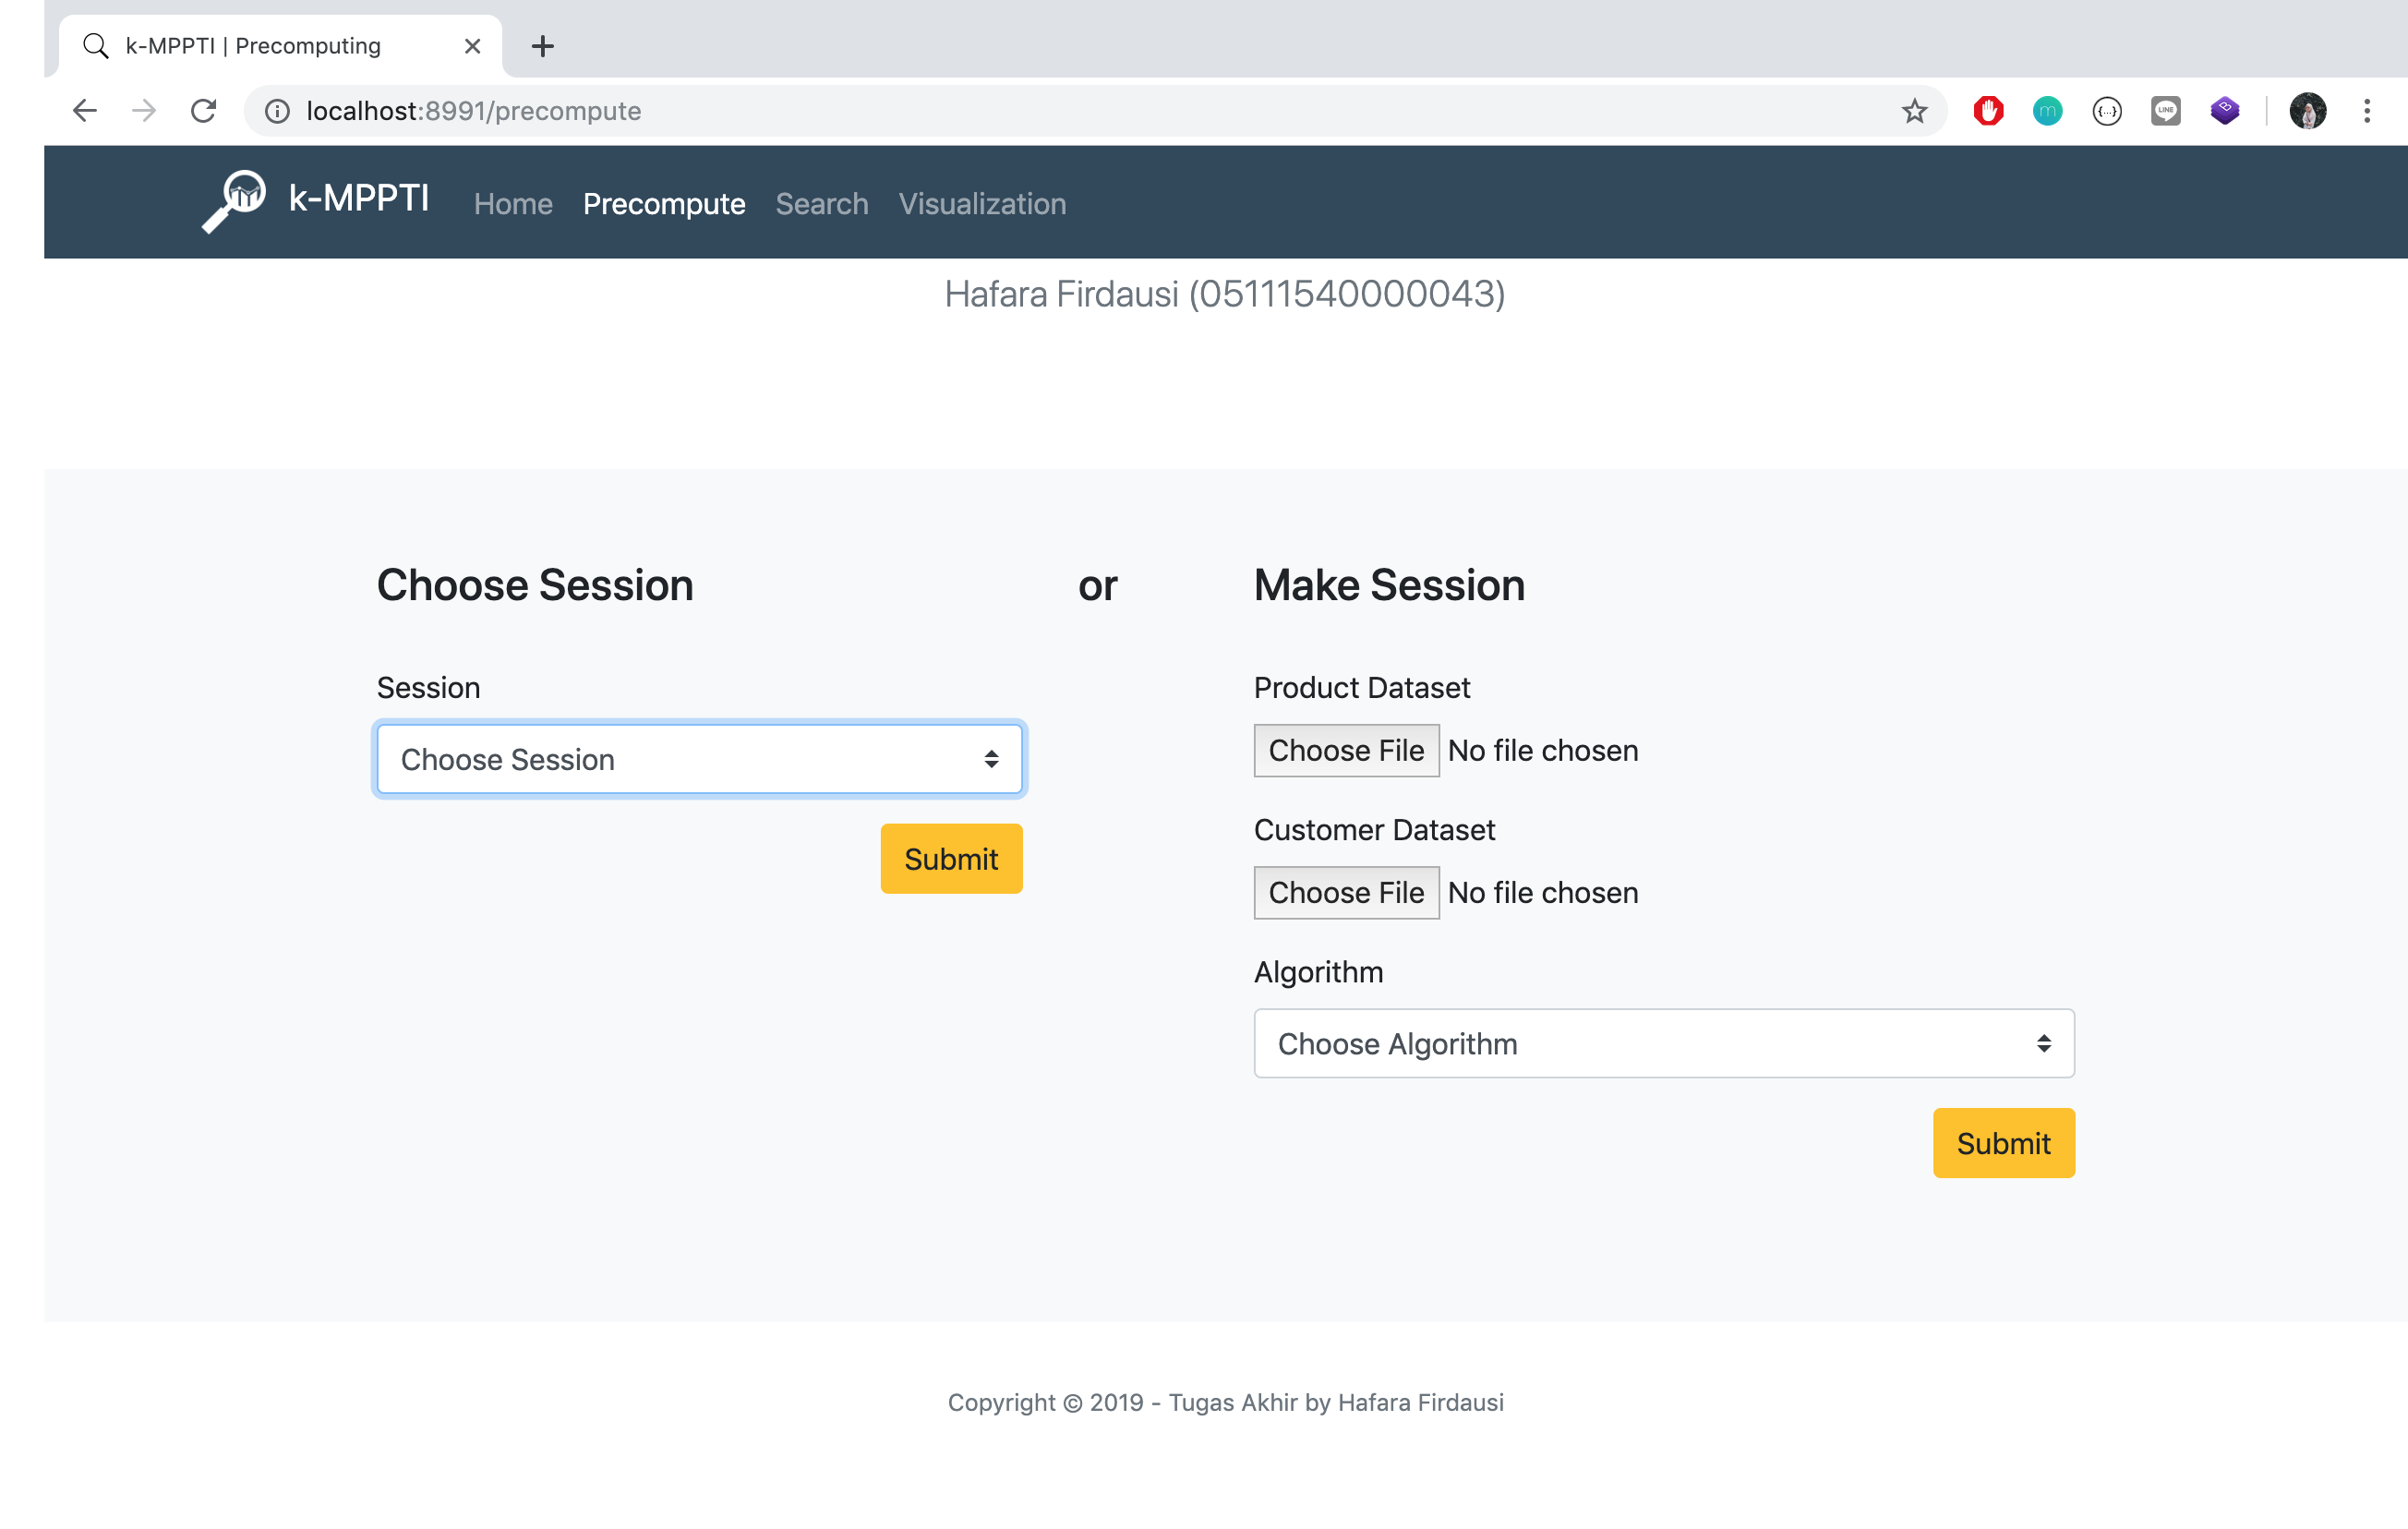
\includegraphics[width=10.5cm]{assets/img/bab4/precompute.png}
	\caption{Implementasi halaman \textit{Precompute}}
	\label{fig:precompute}
\end{figure}

\begin{figure}[H]
	\centering
	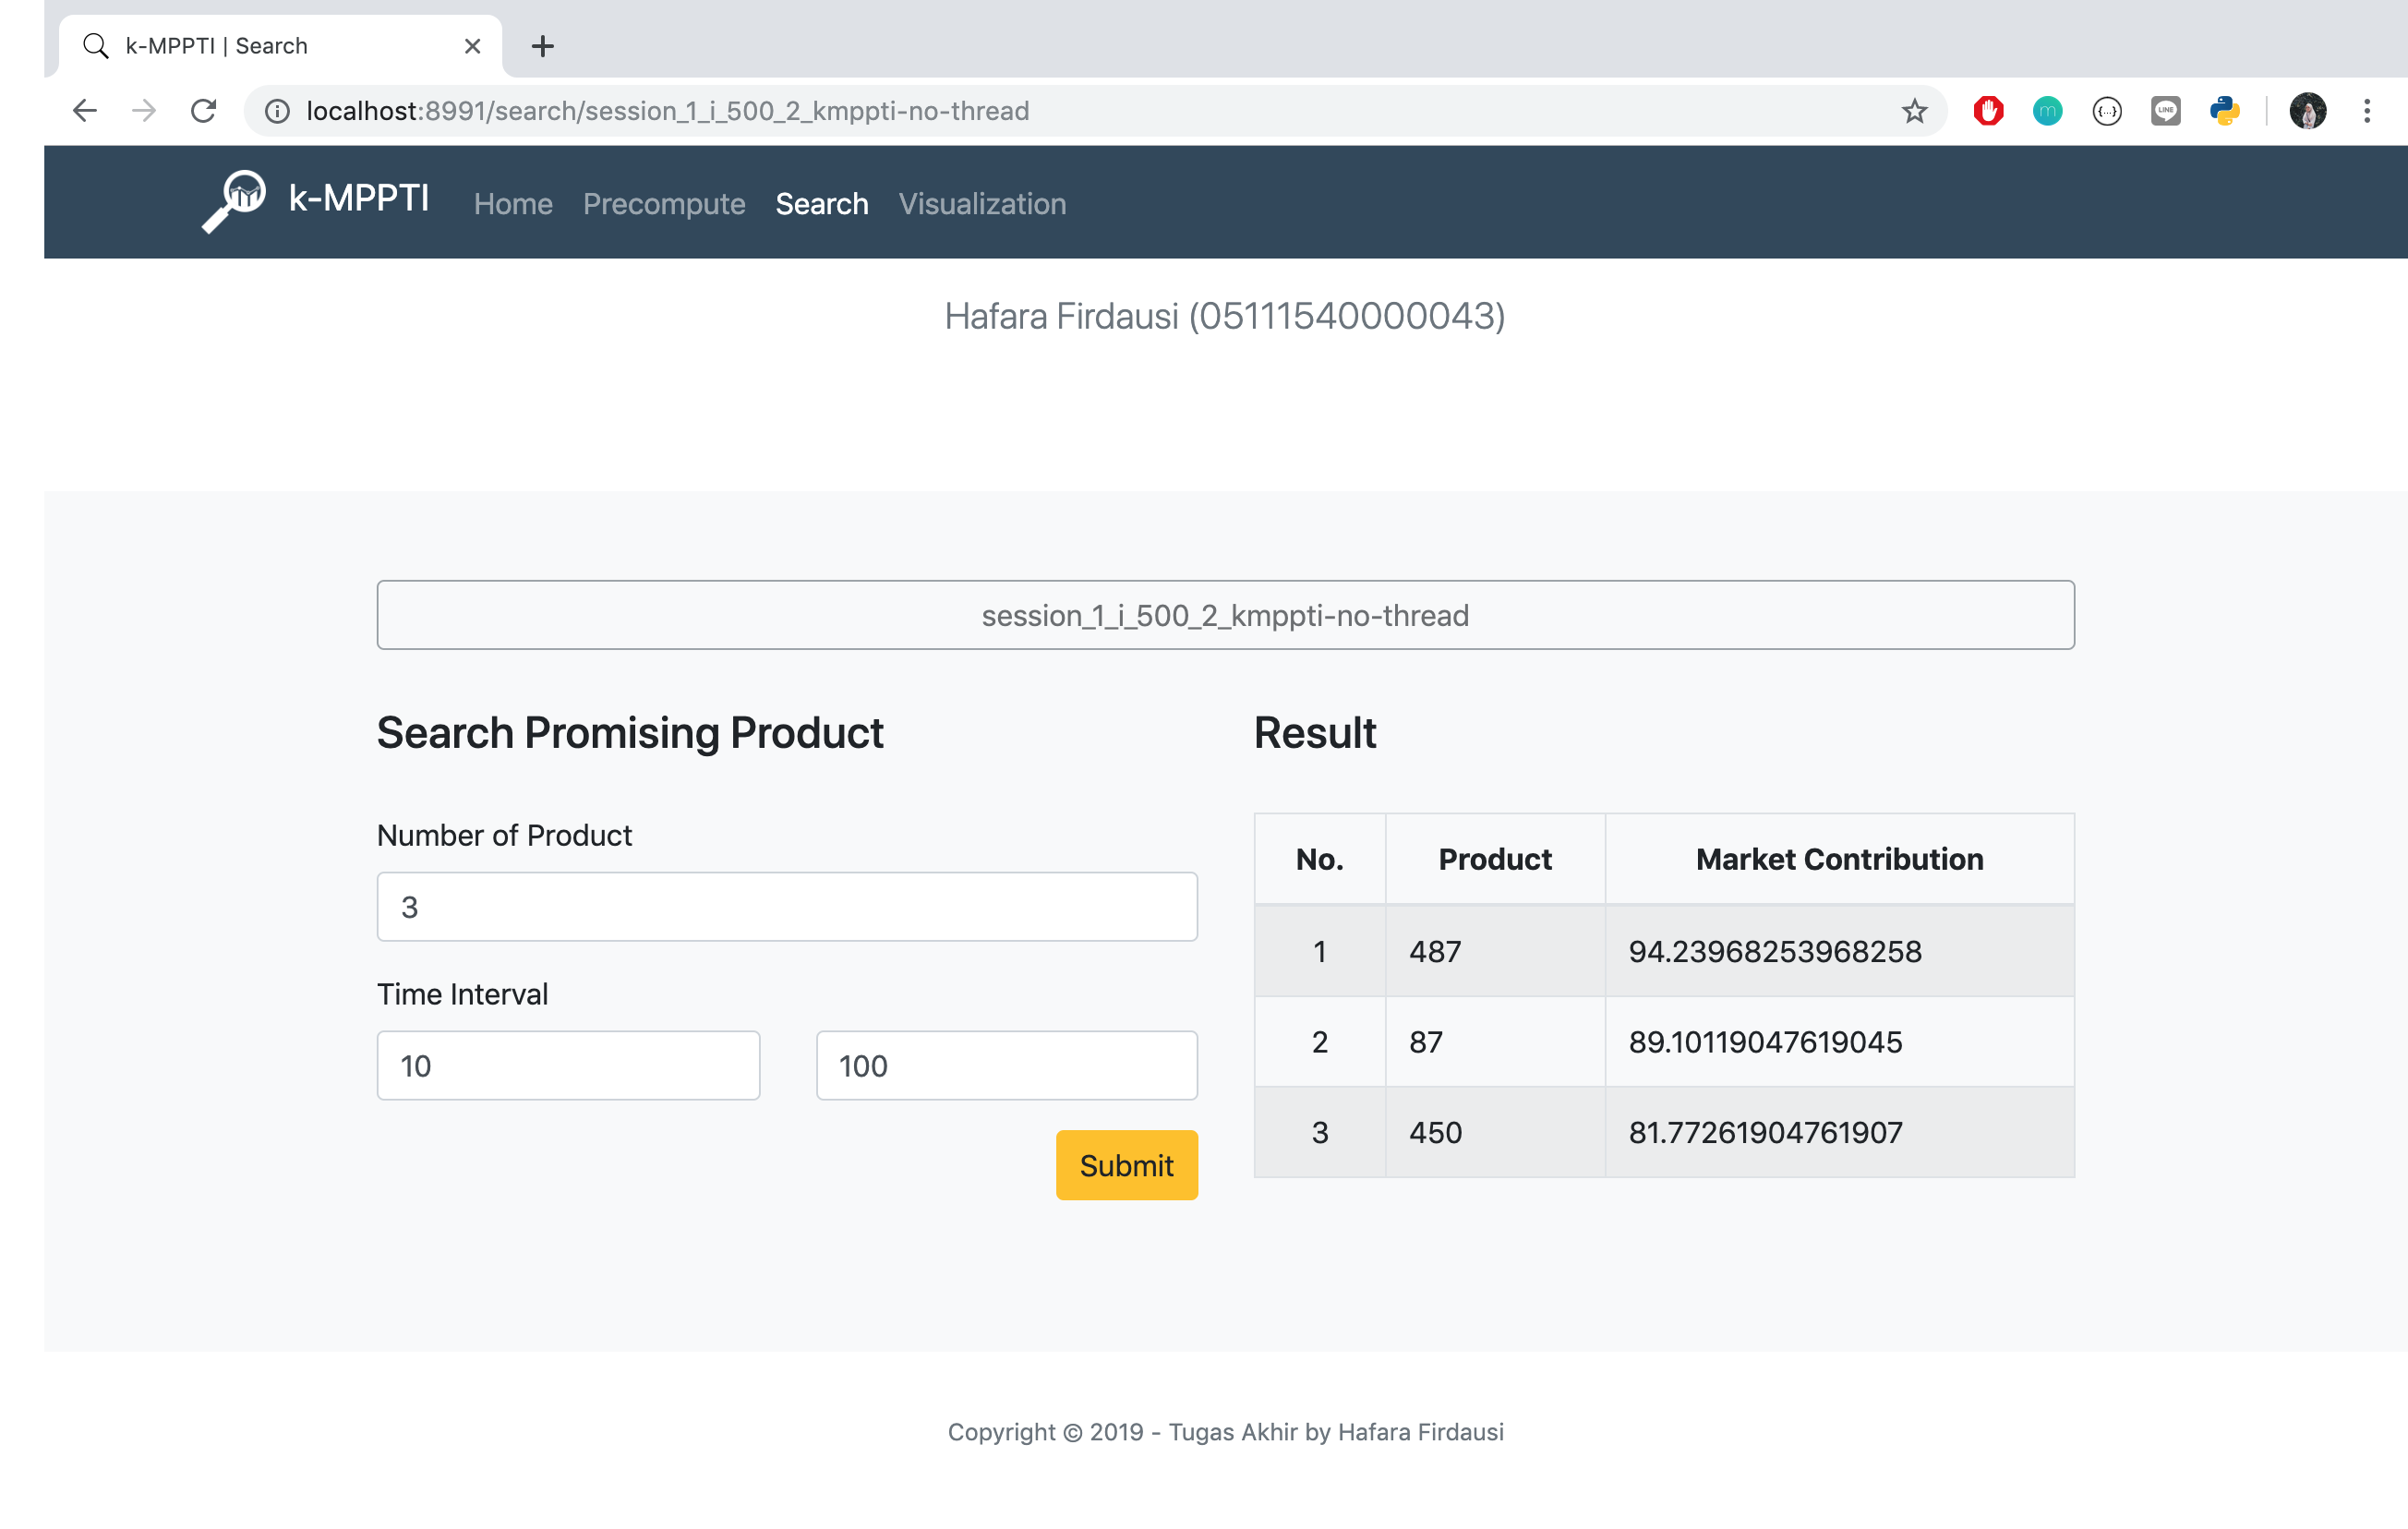
\includegraphics[width=10.5cm]{assets/img/bab4/search.png}
	\caption{Implementasi halaman \textit{Search}}
	\label{fig:search}
\end{figure}

\begin{figure}[H]
	\centering
	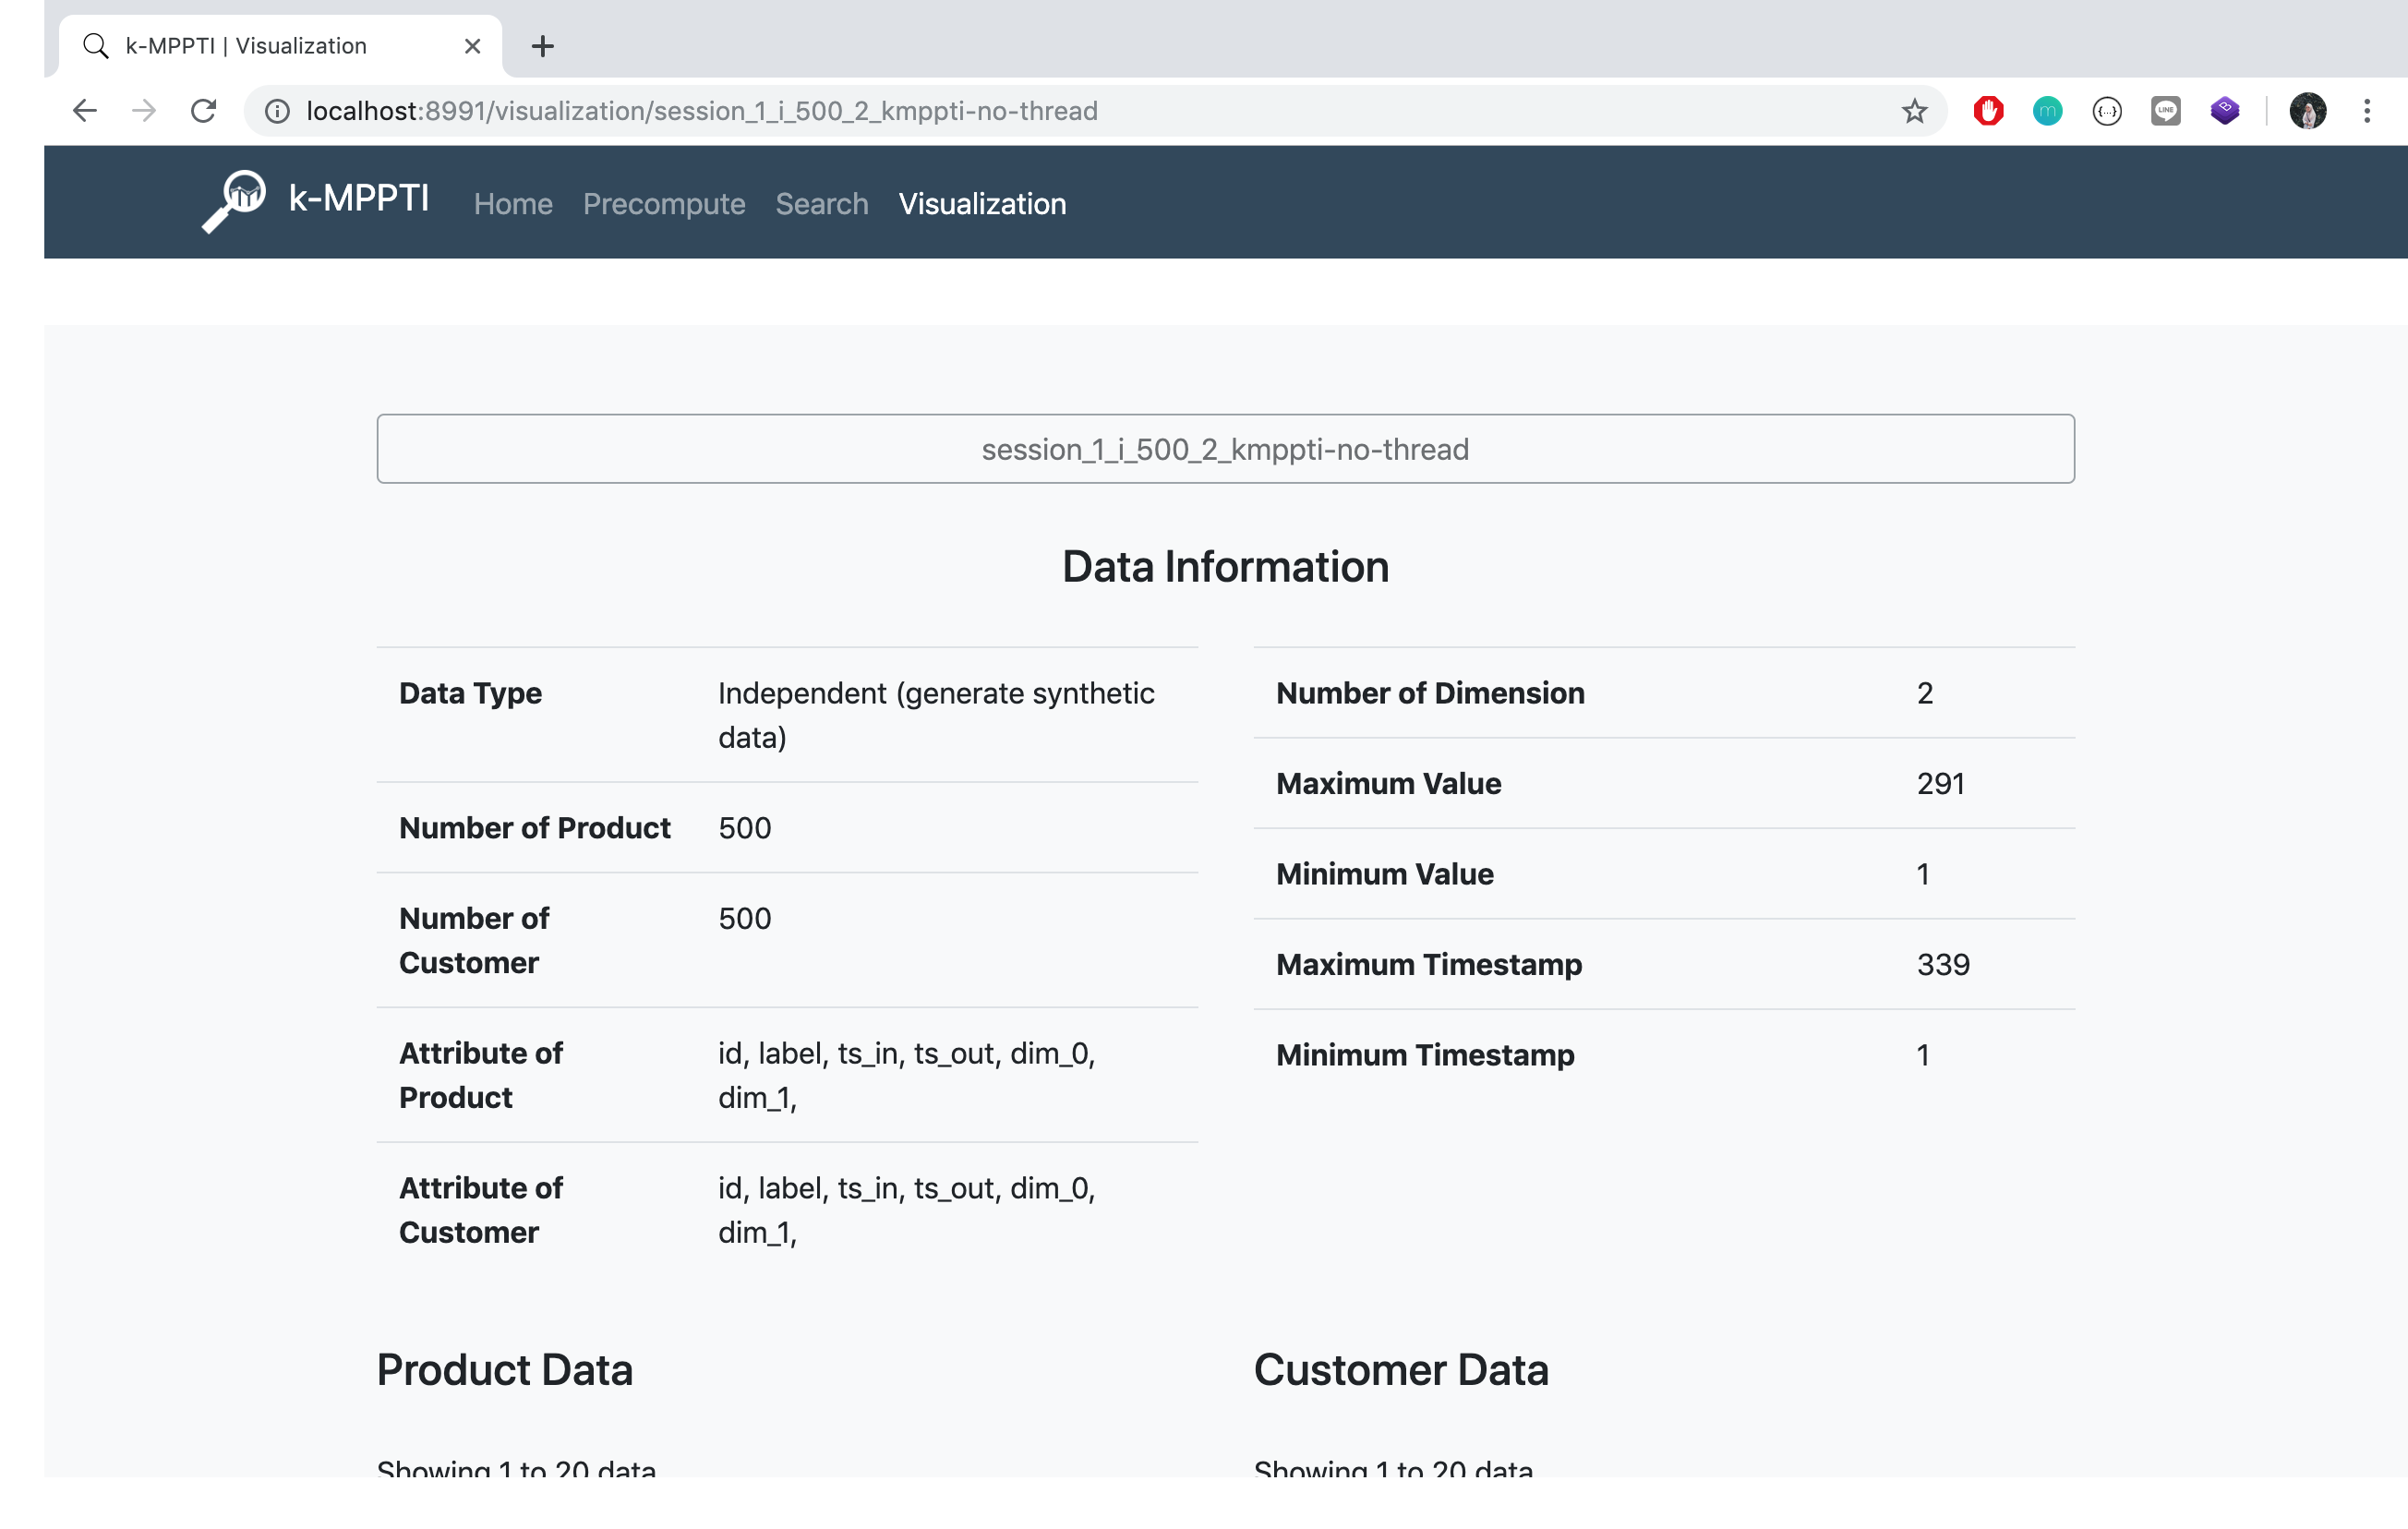
\includegraphics[width=10.5cm]{assets/img/bab4/data-info.png}
	\caption{Implementasi halaman \textit{Visualization} (informasi data)}
	\label{fig:visual-data-info}
\end{figure}

\begin{figure}[H]
	\centering
	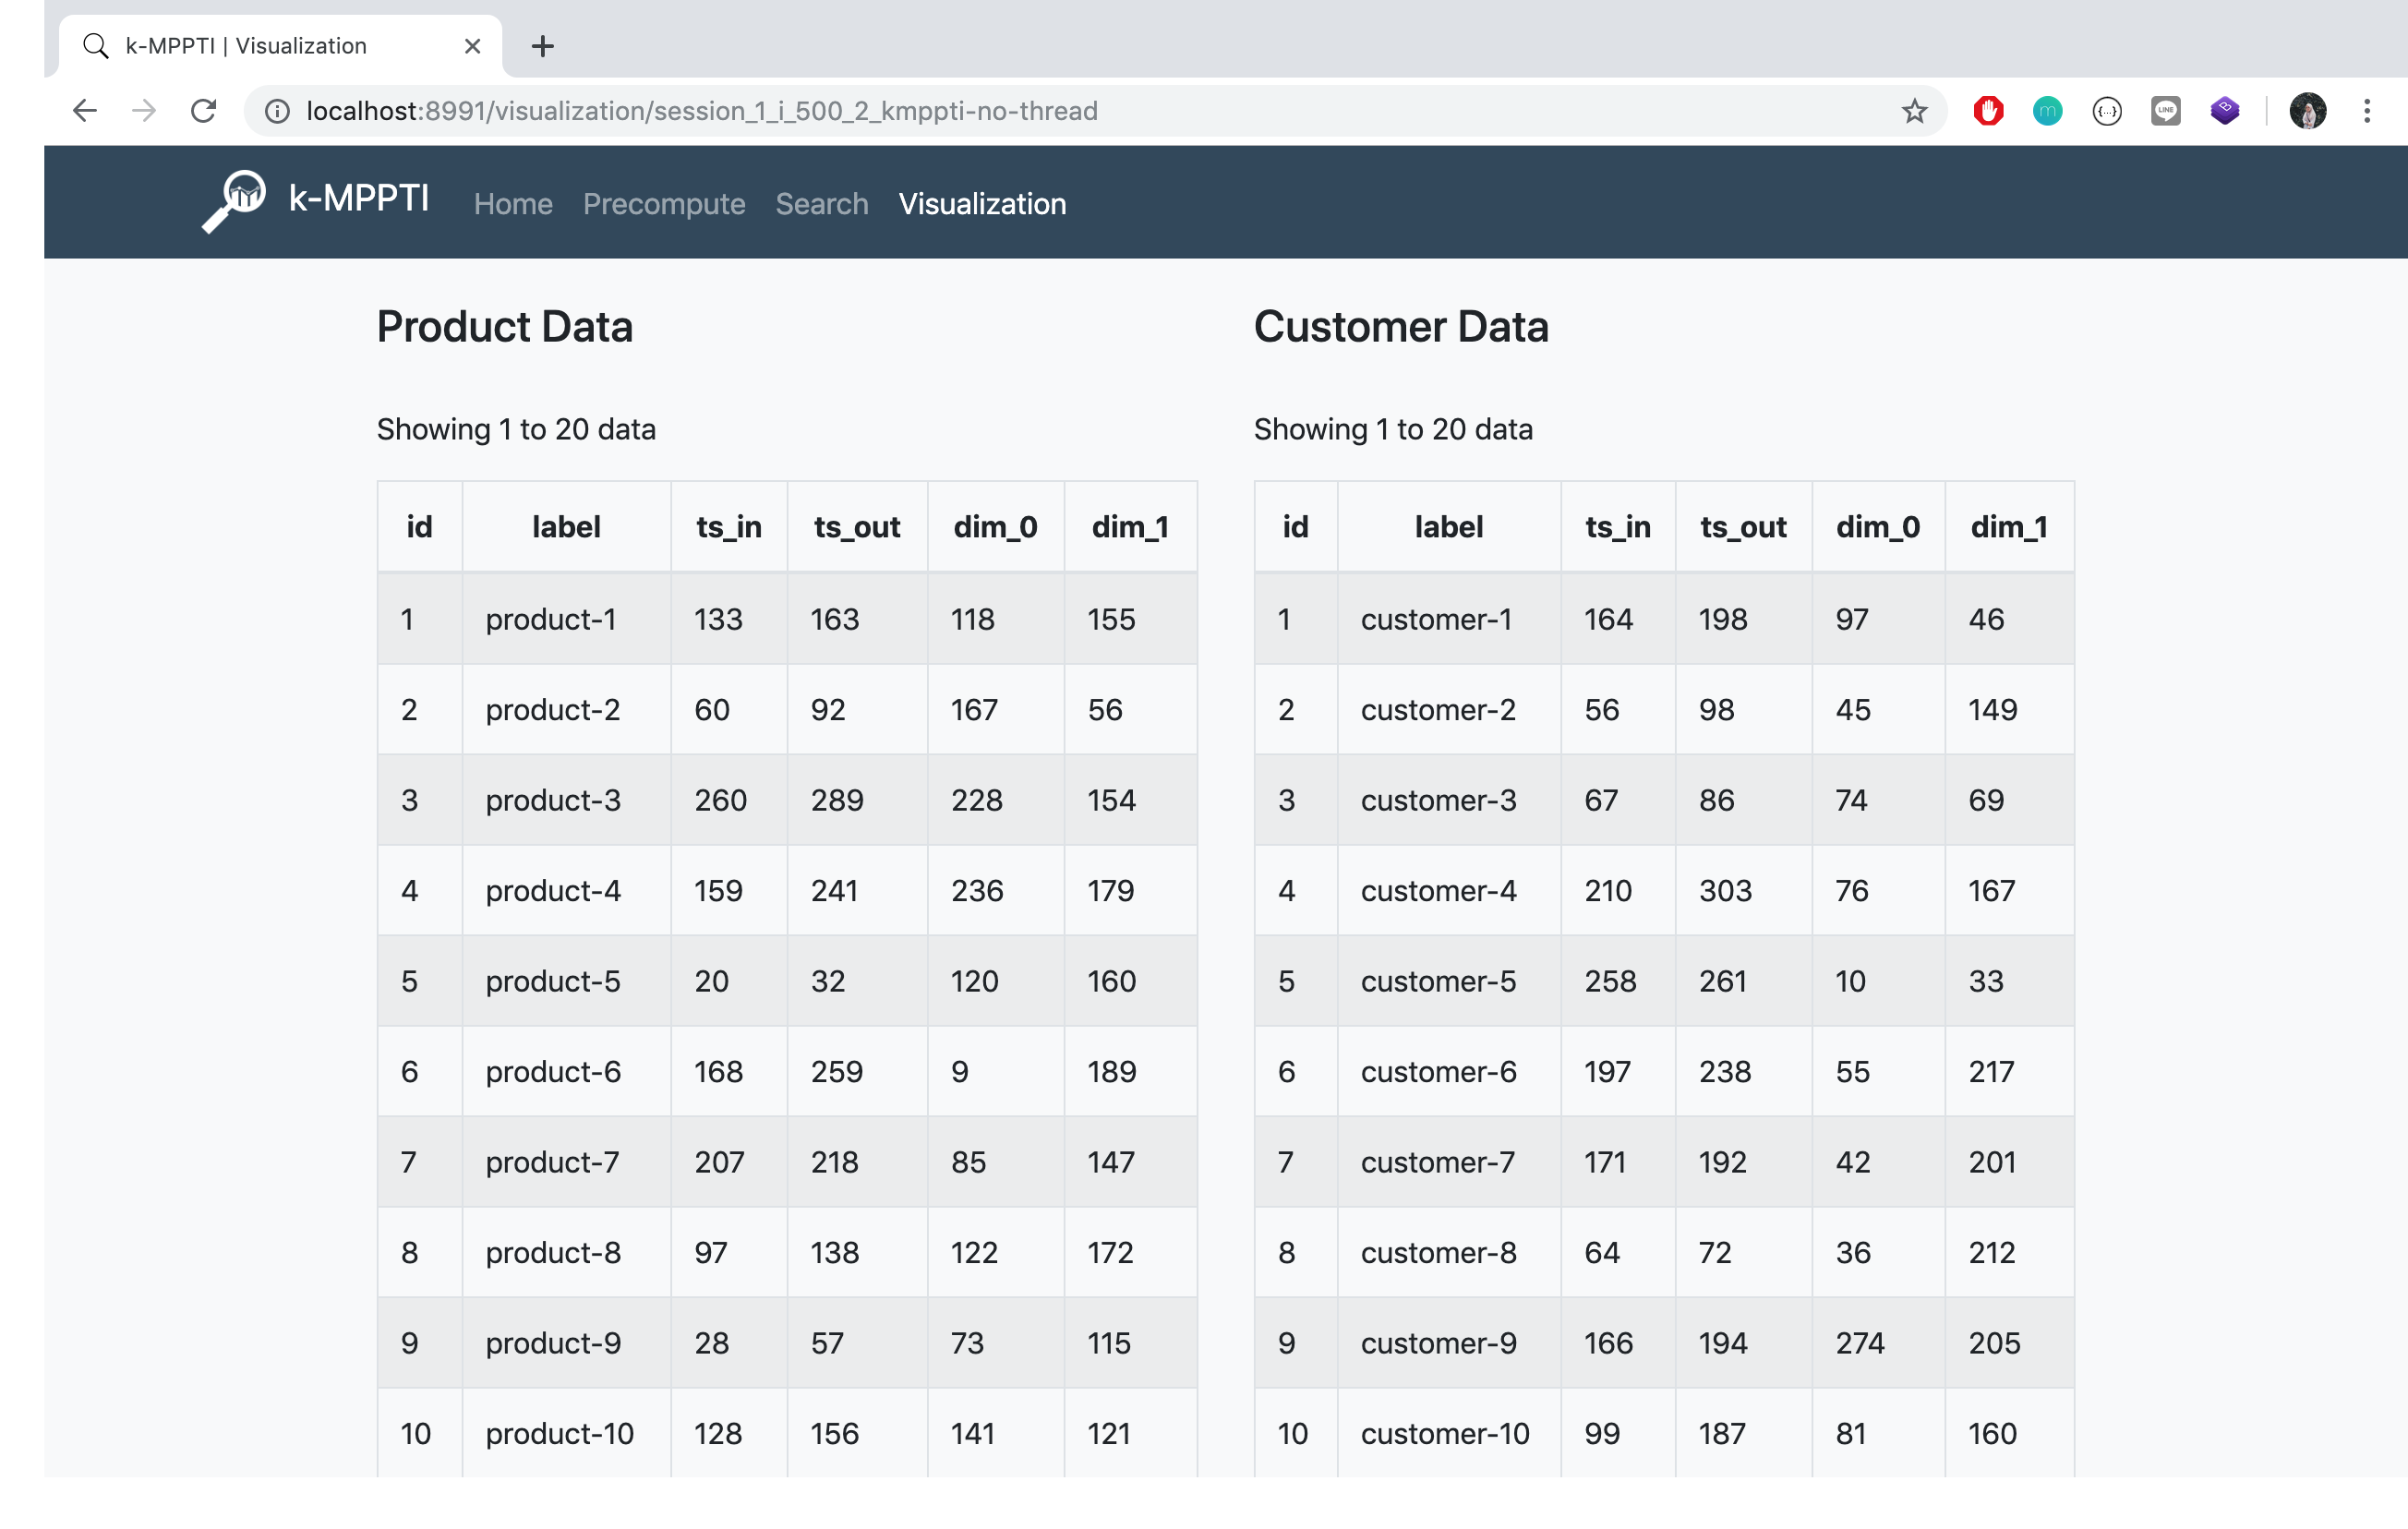
\includegraphics[width=10.5cm]{assets/img/bab4/visual-table.png}
	\caption{Implementasi halaman \textit{Visualization} (pratinjau data)}
	\label{fig:visual-table}
\end{figure}

\begin{figure}[H]
	\centering
	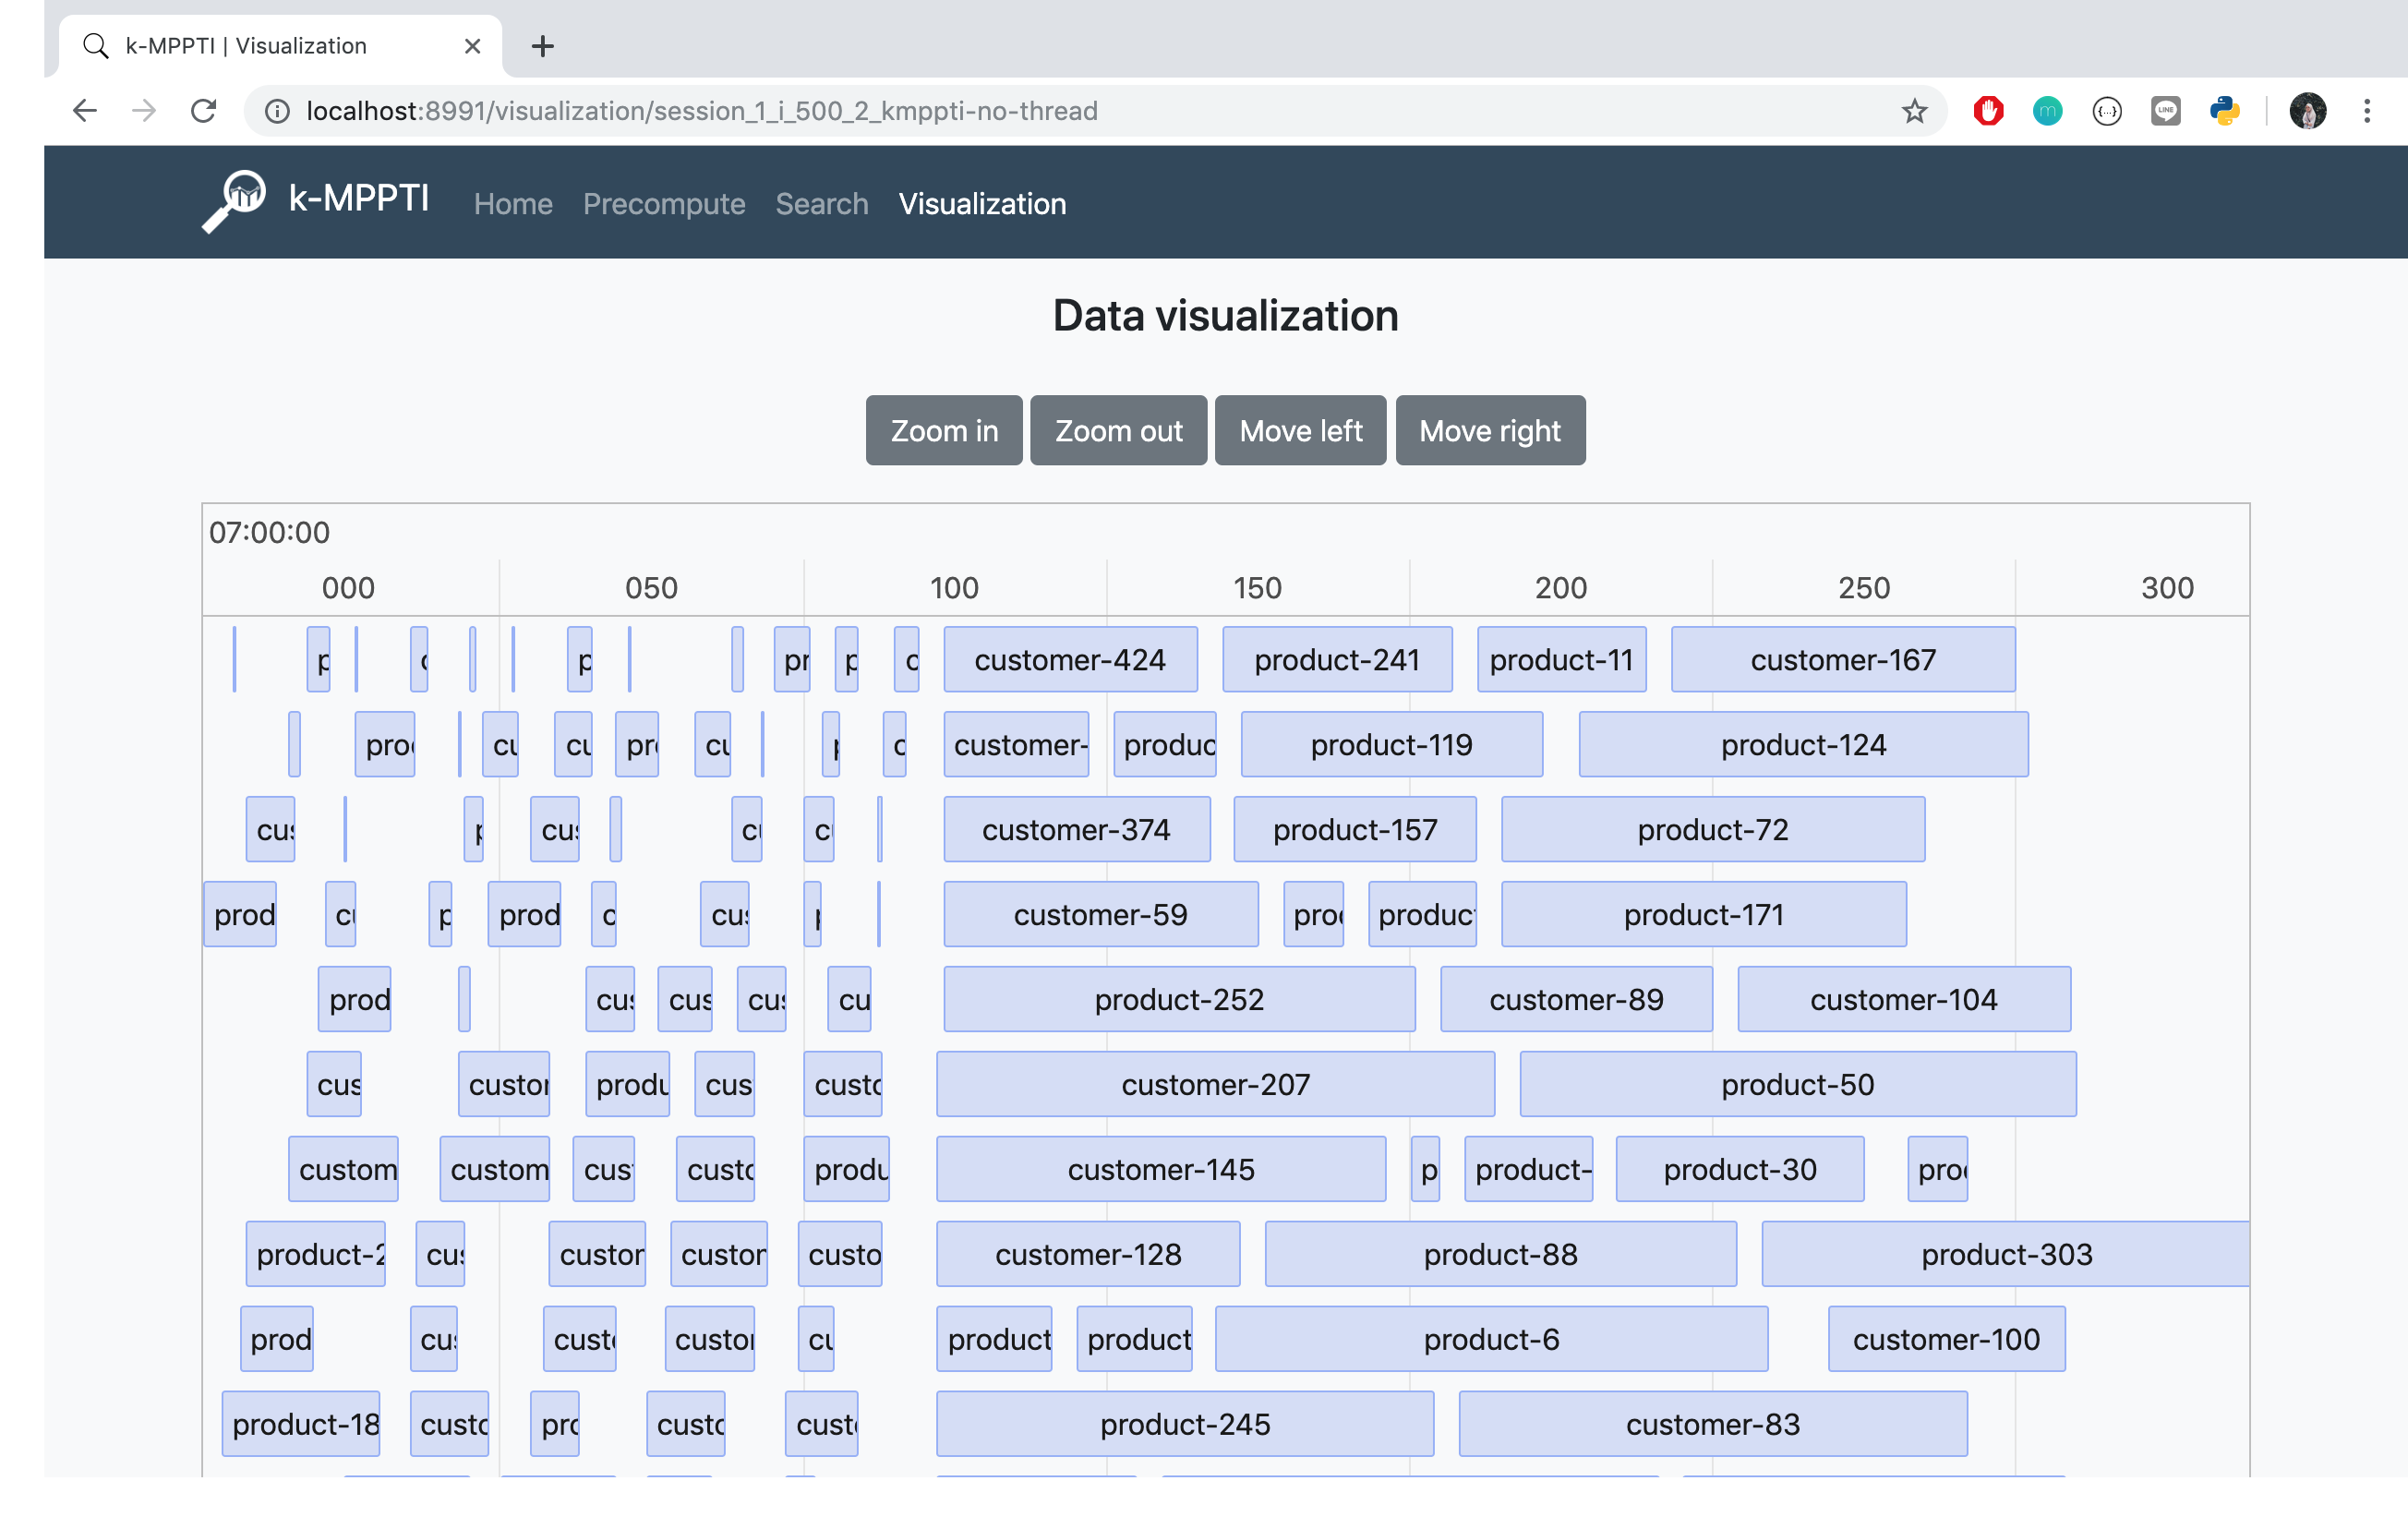
\includegraphics[width=10.5cm]{assets/img/bab4/visual-timeline.png}
	\caption{Implementasi halaman \textit{Visualization} (visualisasi data)}
	\label{fig:visual-timeline}
\end{figure}

Pengguna juga dapat melihat visualisasi data pada menu \textit{"Visualization"} berupa pratinjau data dalam bentuk tabel dan lini masa. Selain itu, pengguna juga dapat melihat informasi detail dari data. Berikut adalah beberapa cuplikan tampilan visualisasi data pada Gambar \ref{fig:visual-data-info}, \ref{fig:visual-table}, dan \ref{fig:visual-timeline}.
